%\clearpage
\section{Innovationsmethoden und Innovationsprozesse}


Ein Innovationsprozesses wird definiert durch die Umsetzung von bestehenden und/oder neuen Erkenntnissen in wirtschaftstaugliche Problemlösungen. Bei den Lösungen handelt es sich meist um ein Produkt oder Dienstleistung, welches oder welche auf dem Markt angeboten wird. Der Erfolg der Lösung hängt jedoch davon ab, ob sie erwartungsgemäss vom Markt aufgenommen wird oder nicht. Der Prozess sollte deshalb nicht nur technisch organisiert werden, sondern muss als interdisziplinären Prozess angesehen werden, welcher alle Unternehmensbereiche darin integriert.

Im Falle eines neuen Produktes, wird Marktforschung betrieben, welche eine Grundlage bietet für das Marketing und die Bedürfnisermittlung an das Endprodukt. Die Forschung- und Entwicklung entwickelt dann gemäss den ermittelten Bedürfnissen das Produkt an sich. Sobald das Produkt auf dem Markt eingeführt wurde, ist der Innovationsprozess bei diesem Beispiel zu Ende.\footnote{Source: https://wirtschaftslexikon.gabler.de/definition/innovationsprozess-41599}



\textbf{« Innovation braucht Methoden »}

Ob es darum geht, Ideen zu finden, ein Problem zu lösen oder zu recherchieren, es kommen jeweils verschiedene Methoden in Frage, um ans Ziel zu kommen. Die kommenden Grafiken sollen dies verdeutlichen. In jedem Arbeitsschritt gibt es eine ausgewählte Gruppe von Menschen, welche diverse Kreativitätstechniken anwenden können (Abb. \ref{fig:Grafik1}\footnote{Source: https://www.lead-innovation.com/hs-fs/hubfs/Vanadyl \%20Seiten/Innovationsprozess/Projektgrafik.\%20Innovationsprozess.jpeg?width=860\& name=Projektgrafik.\%20Innovationsprozess.jpeg}). Diese helfen, dass die Beteiligten für ihren Bereich das Optimum aus beispielsweise Erfahrung oder Kreativität zu Tage führen können. Die gewonnenen Erfahrungen werden jeweils von einer Person verarbeitet und für den nächsten Schritt aufbereitet.

\begin{figure}[h!]
	\centering
	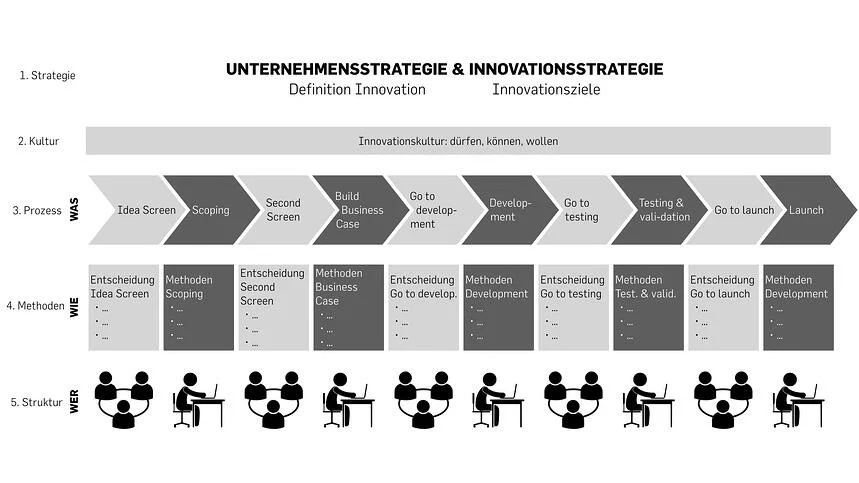
\includegraphics[width=\textwidth]{graphics/Grafik1}
	\caption{Prozessorganisation in einem Betrieb. Ersichtlich, dass während des Innovationsprozesses in verschiedenen Bereichen Methoden angewendet werden. Nach Anwenden der Kreativitätsmethoden werden die gewonnenen Daten jeweils ausgewertet und aufbereitet.}
	\label{fig:Grafik1}
\end{figure} 

Im «Fuzzy Frontend» (Abb. \ref{fig:Grafik2}\footnote{Source: https://www.lead-innovation.com/hs-fs/hubfs/Blogs/Innovationsprozess/Bildschirmfoto\%202017-07-17\%20um\%2016.13.11.png?width=750\& name=Bildschirmfoto\%202017-07-17\%20um\%2016.13.11.png}) ist ersichtlich, dass zwischen Ideenfindung und Konzeptphase die Ideen ständig ausgearbeitet und verbessert werden. Speziell in diesem Bereich ist Kreativität und Innovation von zentraler Bedeutung aber auch die Ideenselektrion spielt eine grosse Rolle. Im weiteren Verlauf des Prozesses sind andere Personen an anderen Prozessen beteiligt, diese sind eher Straight-forward und basieren grösstenteils auf betriebsinternen Erfahrungen. Im Vergleich zum ''Fuzzy Frontend'' arbeiten hier mehr spezialisierte Leute. Dementsprechend ist auch die Breite der Erfahrungsermittlung kleiner.

\begin{figure}[h!]
	\centering
	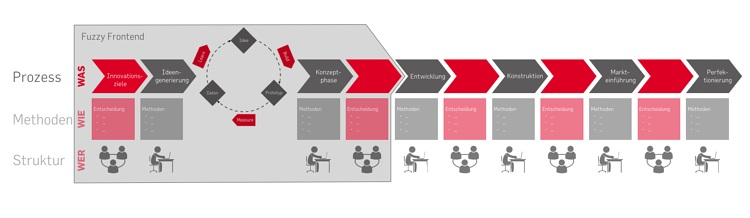
\includegraphics[width=\textwidth]{graphics/Grafik2}
	\caption{Prozesskette während dem Innovationsprozess. Erkennbar das erwähnte ''Fuzzy Frontend'' und die darauf folgenden Prozesse.}
	\label{fig:Grafik2}
\end{figure} 

Beispiel: Die Herstellung einer neuen TV-Geräteserie, die auf den Markt kommen soll. Die Ideenfindung und Konzeption des Gerätes bedarf im Anfangsprozess innovative Kreativitätsmethoden, um Kunden und Lieferanten während dem Vertrieb des Produktes zufrieden stellen zu können und gleichzeitig den betriebsinternen Kapazitäten gerecht zu werden. Ab der Entwicklung sind eher problemlösende Kreativitätsmethoden gefragt. Sobald das Produkt auf dem Markt ist, zeigt sich, ob der Innovationsprozess erfolgreich war.

Es wurde bereits erwähnt, dass ein Innovationsprozess als interdisziplinärer Prozess angesehen werden muss. Je nach Innovationsmethode sind demnach verschiedene Menschen aus verschiedenen Bereichen gefragt. Bei der Entwicklung eines Produktes sind alle Mitarbeiter miteinzubeziehen, von der Putzfrau über die Sekretärin, Ingenieure bishin zum CEO. Jeder sieht das Produkt von einer anderen Seite, worudrch sich ein allgemeineres Bild erstellen lässt. Hier wäre eine 6-3-5 Methode sinnvoll, welche zusätzlich erlaubt die Meinung eines jeden Beteiligten gleich zu gewichten. Geht es darum ein spezifisches technisches Problem zu lösen, sind die Ingenieure gefragt, bei ökonomischen Fragen die Wirtschaftler. Hier wäre eine Brainstorming Methode eher sinnvoll, welche es ermöglicht die zusammenhänge aufzuzeigen und jedem Beteiligten eine sofortige Reaktion zu geben.

Während der Innovationsprozesses gibt es also verschiedene Innovationsmethoden, um das gewünschte Ziel zu erreichen. Eine Innovationsmethode kann aus verschiedenen Kreativitätsmethoden bestehen, die beispielsweise aus Ideenfindung (z.B Brainstorming, 6-3-5) und Ideenselektion (z.B Markttests, Gewichtung, Studien). Im Folgenden werden zwei Kreativitätsmethoden beschrieben, welche in einem Innovationsprozess zur Ideenfindung angewendet werden können.

\newpage

\subsection{6-3-5 Methode}\label{subsec:635Methode}
Die 6-3-5 Methode ist eine Kreativitätstechnik zur Ideenfindung. Optimalerweise wird sie in einem Team mit 6 Personen angewendet. Es können Vorideen entstehen, wie auch gezielte Ideeanareicherung entwickelt werden.
\subsubsection{Vorgehensweise}
\begin{enumerate}

\item In einem ersten Schritt werden jedem Teilenehmer Blätter in Papierform verteilt. Auf den Blättern hat es eine Tabelle mit 3 Spalten und die zuvor definierte Frage. Aus praktischen Gründen sollten sich die Teilnehmer am selben Tisch befinden.
\item Im zweiten Schritt sollte jeder Teilnehmer 3 Ideen zur Grundfrage, also meist eine Lösung für das definierte Problem, in je eine Spalte notieren. Die zeit zum nachdenken ist begrenzt auf 3 Minuten.
\item In einem weiteren Schritt werden die Tabellen weitergegeben und die jeweils zuoberst beschriebenen Ideen können weiterentwickelt werden. Dieser Schritt wird im gesamten 5 mal durchgeführt.

\end{enumerate}

\subsubsection{Vor- und Nachteile}
\begin{tabular}{|l|l|}
	\hline 
	\textbf{Vorteile} & \textbf{Nachteile} \\ 
	\hline 
	Jeder Teilnehmer kann seine Ideen & Keine Zeit für Fragen  \\
	 Notieren, keine dominanten Personen&\\ 
	\hline 
	Somit ist ein Protokoll erfasst&Es können Redundanzen entstehen \\ 
	\hline 
	Es entstehen in kurzer Zeit sehr viele&Arbeitstakt nicht für jeden Teilnehmer gleich\\
	interdisziplinäre Ideen&  \\ 
	\hline 
	Unnötige Diskussionen entfallen&Braucht eine Vorbereitung \\ 
	\hline 
	Jeder Teilnehmer muss sich beteiligen&  \\ 
	\hline 
\end{tabular} 
\subsubsection{Beispiel}
\begin{figure}[H]
	\centering
	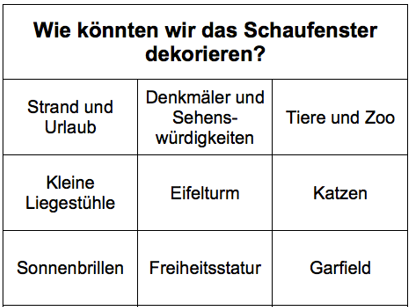
\includegraphics[width=0.5\textwidth]{M635.png}
	\caption{In dieser Abbildung kann erkannt werden, wie Ideen zur Frage: dekoration des Schafensters, entstanden sind}
	%\cite{thirah_vorhangeschloss-schlussel-computer-icons_nodate}
	%\raggedleft
\end{figure}
\newpage
\subsection{Brainstorming}\label{subsec:Brainstorming}

Eine sehr bewährte Variante der Ideenfindung stellt das Brainstorming dar. Hauptsächlich geht es darum, aus möglichst vielen Ideen die besten Ergebnisse herauszufiltern und zu kombinieren. Brainstorming wird am besten in kleineren Gruppen durchgeführt. Wird es in grösseren Gruppen durchgeführt, so entsteht schnell Chaos.

\subsubsection{Vorgehensweise}

\begin{enumerate}
\item In einem ersten Schritt wird ein Moderator erwählt, welcher die Ideen zusammenträgt und diese für alle sichtbar aufschreibt. Alternativ kann auch eine Wandtafel benutzt werden, auf welche jeder seine Ideen aufschreiben kann.
\item In einem zweiten Schritt werden Ideen gesammelt. Dabei kann jeder seine Ideen in einer offenen Runde frei dem Moderator mitteilen oder auf die Tafel schreiben. Dies gewährleistet, dass aus bereits genannten Ideen auch neue Ideen entstehen können. Ein wichtiger Punkt dabei ist, dass keine Idee zu abwegig ist.
\item In einem letzten Schritt werden dann die Ideen sortiert und ausgewertet. Die Teilnehmer sortieren gemeinsam die Ideen und filtern die besten Ideen heraus. Aus diesen Ideen entsteht dann die Zielidee. 

\end{enumerate}
\subsubsection{Vor- und Nachteile}

\begin{tabular}{|l|l|}
	\hline 
	\textbf{Vorteile} & \textbf{Nachteile} \\ 
	\hline 
	Frei Kreativität für jeden & Schwierige Handabung für den Moderator  \\
	\hline 
	Schnelle Ideenfindung & Potential für zu viel input \\ 
	\hline 
	Einbezug aller anwesenden Teilnehmer & Belustigung einzelner bei \flqq abwegigen\frqq  Ideen\\
	\hline
\end{tabular} 


\begin{figure}[h!]
	\centering
	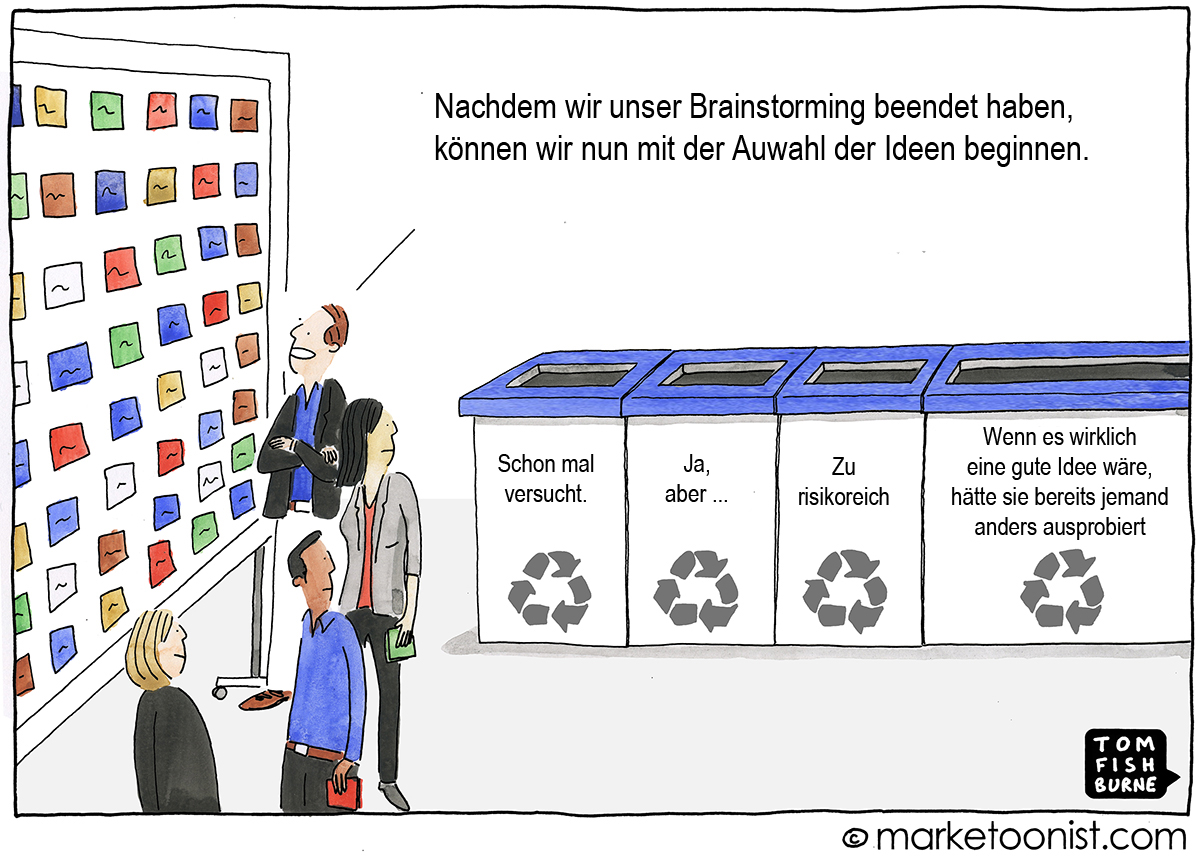
\includegraphics[width=0.8\textwidth]{graphics/Brain}
	\caption{Anschauungsbild Brainstorming}
	\label{fig:Brainstorming}
\end{figure} 




  

